\chapter{Learning Dynamical Systems via Optimal Transport and Stochastic Control}
\label{cha:neural_sde}

\dictum[Erwin Schr\"odinger, \textit{What is Life?} (1944)]{%
  Living matter evades the decay to equilibrium.}%


\section{Diffusion Schr\"odinger Bridges}





\section{Data-Driven Priors for Diffusion Schr\"odinger Bridges}

The \acrfull{SB} \citep{leonard2013survey, chen2021stochastic}, alternatively known as the \emph{dynamic} entropy-regularized \acrlong{OT} (OT), has recently received significant attention from the machine learning community. In contrast to the classical \emph{static} \acrshort{OT} where one seeks a {coupling} between measures that minimizes the average cost \citep{villani2009optimal, peyre2019computational}, the goal of \acrshortpl{SB} is to find the optimal \emph{stochastic processes} that evolve a given measure into another. As such, \acrshortpl{SB} are particularly suitable for learning complex continuous-time systems, and have been successfully applied to a wide range of applications such as sampling \citep{bernton2019schr, huang2021schrodinger}, generative modeling \citep{chen2021likelihood,de2021diffusion,wang2021deep}, molecular biology \citep{holdijk2022path}, and mean-field games \citep{liu2022deep}. 

%The \emph{static} optimal transport (OT) problems seek to find the optimal mapping which transforms a given probability measure into another while minimizing the 

%Comparing between probability measures is ubiquitous in machine learning, for which 
%Optimal transport (OT) and entropy-regularized \acrshort{OT} problems play a pivotal role in machine learning \citep{villani2009optimal, peyre2019computational}, where one seeks a \emph{mapping} that transports between measures while minimizing the average cost. In recent years, there is a rapid growth of interest in solving the \emph{dynamical} extensions of these \acrshort{OT} problems, i.e., finding the optimal \emph{trajectories} that transport measures, with applications ranging from sampling and generative modeling \citep{} to molecular dynamics and mean-field games \citep{}. In the literature, these dynamical \acrshort{OT} problems are known as the \acrfull{SB} \citep{leonard2013survey, chen2021stochastic} due to an equivalent formulation that dates back to \citep{schrodinger1931umkehrung, schrodinger1932theorie}.

%the dynamic extensions of these \acrshort{OT} problems, i.e., finding the optimal \emph{trajectories} that transport measures, have witnessed a sudden surge of interest. A particularly prominent instance of these extensions is the \acrfull{SB} \citep{schrodinger1931umkehrung, schrodinger1932theorie}, for comparing constrained \emph{stochastic processes} has attracted significant attention. Creative applications of \acrshort{SB} have already yielded success in sampling and generative modeling tasks \citep{}, while also witnessing a surging interest in fields like molecular dynamics and mean-field games \citep{}. 

\begin{figure}
    \centering
    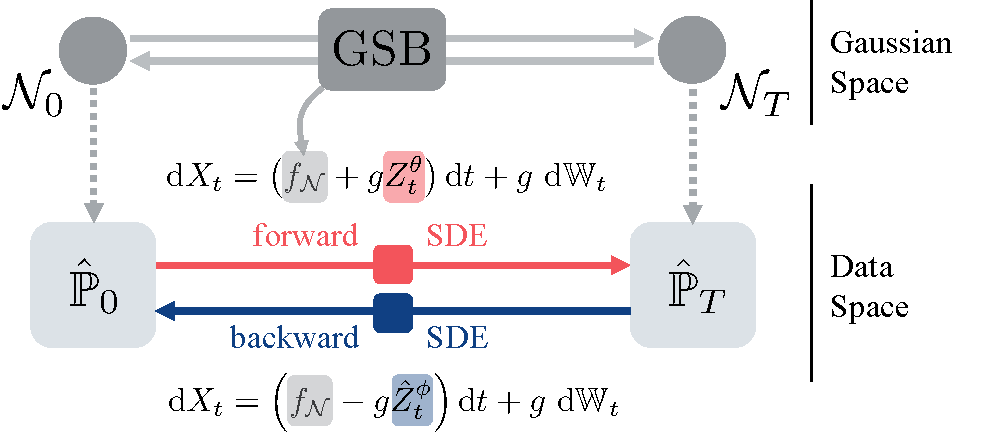
\includegraphics[width=1.1\linewidth]{figures/fig_overview_gsb.pdf}
    \caption{Solving the \acrshort{SB} problem between $\distinit$ and $\distend$ is notoriously difficult because it requires learning the time-dependent drifts of two SDEs that respect the desired marginals, and a random initialization for these drifts is usually extremely far from satisfying that constraint. We propose a data-dependent procedure that relies first on Gaussian approximations of the data measures, which provide a closed-form drift $f_{\mathcal{N}}$ in \eqref{eq:GSB-forward} (the \acrshort{GSB}). We show that this facilitates the training of forward/backward drifts $\hat{Z}^\theta_t, \hat{Z}^\phi_t$.}%
    \label{fig:overview}
\end{figure}

Despite of these impressive achievements, a common limitation of the existing works is that the \acrshortpl{SB} are typically solved in a purely {numerical} fashion. In sharp contrast, it is well-known that many important \acrshort{OT} problems for \emph{Gaussian} measures admit \emph{closed-form} solutions, and the advantages of such solutions are numerous: they have inspired new learning methods \citep{rabin2011wasserstein, vayer2019sliced, bonneel2015sliced}, they can serve as the ground truth for evaluating numerical schemes \citep{janati2020entropic}, and they have lead to the discovery of a new geometry that is both rich in theory and application \citep{takatsu2010wasserstein}. 

\newpage
The goal of our paper is to continue this pursuit of closed-form solutions and thereby extending these advantages to \acrshort{SB}-based learning methods. For an overview of the method, see Fig.~\ref{fig:overview}. To this end, we make the following \textbf{contributions}: \vspace{8pt}
%As a central contribution, we derive a set of new expressions for \acrfullp{GSB}, i.e.,\acrshortpl{SB} between Gaussian measures, that covers a wide range of applications. Furthermore, our analysis reveals a
\begin{enumerate}[leftmargin=.4cm,itemsep=.0cm,topsep=.0cm]
\item As our central result, we derive the closed-form expressions for \acrfullpl{GSB}, i.e.,\acrshortpl{SB} between Gaussian measures. This is a challenging task for which all existing techniques fail, and thus we need to resort to a number of new ideas from entropic \acrshort{OT}, Riemannian geometry, and generator theory; see \cref{sec:overview}.
%, thereby filling the void of. %, that covers a wide range of applications.  %These formulas constitute the first non-trivial closed forms for \emph{dynamic} entropy-regularized \acrshort{OT}. %The proof combines a number of ideas from entropic optimal transport, Riemannian geometry, Gaussian analysis, and generator theory, which might be of independent interest; see \crefrange{sec:mechanics}{sec:results}.

\item We extend the deep connection between geometry and Gaussian \acrshort{OT} to \acrlongpl{GSB}. In particular, our results can be seen as a vast generalization of the classical Bures-Wasserstein geodesics between Gaussian measures \citep{takatsu2010wasserstein, bhatia2019bures}, which is the foundation of many computational methods \citep{chewi2020gradient, altschuler2021averaging, han2021riemannian}.

\item Via a simple Gaussian approximation on real \emph{single-cell genomics} data, we numerically demonstrate that many benefits of the closed-form expressions in static \acrshort{OT} immediately carry over to \acrshort{SB}-based learning methods: We report improved numerical stability and tuning insensitivity when trained on benchmark datasets, which ultimately lead to an overall better performance.

\end{enumerate}


\subsection{Preliminaries on Gaussian Optimal Transport Problems}


Throughout this paper, let $\xi \sim \Ncal(\mu, \Sigma)$ and $\xi' \sim \Ncal(\mu', \Sigma')$ denote two given Gaussian random variables. By abusing the notation, we will continue to denote the measures of these Gaussians by $\xi$ and $\xi'$, respectively. We will also denote by $\Pi(\xi,\xi')$ the set of all their couplings. 


\subsubsection{Static Gaussian Optimal Transport}
\label{sec:staticGOT}
The \emph{static} entropy-regularized \acrshort{OT} between Gaussians refers to the following minimization problem \citep{peyre2019computational}:
% An important class of problems which generalizes \eqref{eq:W2Gaussian}, is the static entropy-regularized \acrshort{OT} between Gaussians:
\begin{equation}
\label{eq:RegW2Gaussian}
%\tag{OT$_\sigma$}
\min_{\coupling \in \Coupling(\xi, \xi')} \int  \norm{\point-\pointalt}^2  \drm \coupling(\point, \pointalt) + 2\sigma^2 \KL{\pi}{ \xi \otimes \xi'  },
\end{equation}where $\xi\otimes\xi'$ denotes the product measure of $\xi$ and $\xi'$, and $\sigma \geq 0$ is a regularization parameter. When $\sigma = 0$, \eqref{eq:RegW2Gaussian} reduces to the classical 2-Wasserstein distance between $\xi$ and $\xi'$ \citep{villani2009optimal}, whose closed-form solution is classical \citep{dowson1982frechet, olkin1982distance}. The case for general $\sigma$ is more involved, and an analytical expression was only recently found \citep{bojilov2016matching, del2020statistical, janati2020entropic, mallasto2021entropy}: Setting% the specific form is quite convoluted, and thus we defer it to \cref{app:GaussianSB}.
\begin{equation}
\label{eq:Cstar}
D_\sigma \defeq \parens{ 4\Sigma^{\frac{1}{2}} \Sigma' \Sigma^{\frac{1}{2}} +  \sigma^4\eye  }^{\frac{1}{2}},\quad C_\sigma \defeq \frac{1}{2}\parens{\Sigma^{\frac{1}{2}} D_\sigma \Sigma^{-\frac{1}{2}} - \sigma^2\eye},
\end{equation}
then the solution $\pi^\star$ to \eqref{eq:RegW2Gaussian} is itself a Gaussian:
\begin{align}
\label{eq:StaticGaussianSB-sol}
\pi^\star \sim \Ncal \parens*{  \begin{bmatrix}
\mu \\
\mu'
\end{bmatrix},  \begin{bmatrix}
\Sigma&C_\sigma\\
C_\sigma^\top&\Sigma'
\end{bmatrix}}.
\end{align}

\subsubsection{Dynamic Gaussian Optimal Transport}
\label{sec:dynamicGOT-BB}


In the literature, \eqref{eq:RegW2Gaussian} is commonly referred to as the \emph{static} \acrshort{OT} formulation, since it merely asks \emph{where} the mass should be transported to (i.e., $\pi(\point,\pointalt)$ dictates how much mass at $\point$ should be transported to $\pointalt$). In contrast, the more general problem of \emph{dynamic} Gaussian \acrshort{OT} seeks to answer \emph{how} the mass the should be transported:
\begin{align}
\label{eq:BBGaussian}
%\tag{dyn-OT$_\sigma$}
\min_{\ssstyle\substack{{\measure[0] = \xi,\ \measure[\horizon] = \xi'}}} \exof*{\int_{0}^\horizon  \frac{1}{2} \norm{\vect}^2 + \frac{\sigma^4}{8} \norm*{\nabla\log\measure}^2 \dt}.
\end{align}Here, the minimization is taken over all pairs $(\measure, \vect)$ where $\measure$ is an absolutely continuous curve of measures \citep{ambrosio2006gradient}, and $\vect:\R^\vdim\to\R^\vdim$ is such that the continuity equation holds:
\begin{equation}
\label{eq:Coneq}
\pt\measure = - \Div(\measure \vect),
\end{equation}
where $\left(\Div \vect\right)(\point) \coloneqq \sum_{i=1}^d \frac{\partial}{\partial \point_i}v_t^{i}(\point)$ denotes the divergence operator with respect to the $\point$ variable. It can be shown that, if $\rho^\star_t$ is the optimal curve for \eqref{eq:BBGaussian}, then the joint distribution of the end marginals $(\rho^\star_0, \rho_1^\star)$ coincides with \eqref{eq:StaticGaussianSB-sol}, hence the interpretation of $\rho_t^\star$ as the optimal \emph{trajectory} in the space of measures  \citep{chen2016relation, gentil2017analogy, chen2021stochastic, gentil2020dynamical}.

To our knowledge, the only work that has partially addressed the closed-form solution of \eqref{eq:BBGaussian} is \citet{mallasto2021entropy}, whose results are nonetheless insufficient to cover important applications such as generative modeling. In \cref{sec:results}, we will derive a vast generalization of the results in \citet{mallasto2021entropy} and provide a detailed comparison in \crefrange{sec:overview}{sec:mechanics}.


\subsection{The Gaussian Schr\"odinger Bridge Problem and Analysis Overview}

\newcommand{\Pstar}[1][\ctime]{\mathbb{P}^\star_{#1}}

The purpose of this section is to introduce the core objectives in our paper, the \acrlongpl{GSB}, and establish their connection to the Gaussian \acrshort{OT} problems in \cref{sec:prelim}. To help the reader navigate our somewhat technical proofs in \crefrange{sec:mechanics}{sec:results},  we illustrate in \cref{sec:tere} the high-level challenges as well as our new techniques for solving \acrlongpl{GSB}.

\subsubsection{Schr\"odinger Bridges as Dynamic Entropy-Regularized Optimal Transport}


Let $\nu, \nu'$ be two given measures and let $\refpro$ be an arbitrary stochastic process. In its most generic form, the \acrlong{SB} refers to the following constrained KL-minimization problem over all stochastic processes $\Pmargin$ \citep{leonard2013survey, chen2021stochastic}: 
\begin{equation}
\label{eq:SB}
%\tag{SB}
\min_{ \substack{ \Pinit = \nu, \; \Pend = \nu'} } \KL{\Pmargin}{\refpro}.% \quad \sigma >0 \textup{ and \Wiener
\end{equation}


In practice, $\nu$ and $\nu'$ typically arise as the (empirical) \emph{marginal} distributions of a complicated continuous-time dynamics observed at the starting and end times, and $\refpro$ is a ``prior process'' representing our belief of the dynamics before observing any data. The solution $\Pstar$ to \eqref{eq:SB} is thus interpreted as the best dynamics that conforms to the prior belief $\refpro$ while respecting the data marginals ($\Pstar[0] = \nu, \Pstar[\horizon] = \nu'$). 

In this paper, we will consider a general class of $\refpro$'s that includes most existing processes in the machine learning applications of \acrshortpl{SB}. Specifically, with some initial condition $\refsde[0]$, we will take $\refpro$ to be the measure of the linear \acrfull{SDE}:
% To facilitate the numerical solutions of \eqref{eq:SB}, $\refpro$ is typically chosen so that conditional distributions given initial points admit a simple expression. To this end, we will consider the following general class of \acrfullp{SDE} which incorporates, to our knowledge, all the existing processes in the literature: With some initial condition $\refsde[0]$, take $\refpro$ to be the measure of
\begin{equation}
\label{eq:linearsde}
\drefsde = \parens*{\drift \refsde  + \shift }\dd t + \volat \dWiener[\ctime] \defeq \driftf\dt + \volat \dWiener[\ctime].
\end{equation}
Here, $\drift: \R^+ \to \R$, $\shift : \R^+ \to \R^\vdim$, and $\volat: \R^+ \to \R^+$ are smooth functions. In this case, \acrshortpl{SB} can be seen as generalized dynamical \acrshort{OT} between two (not necessarily Gaussian) measures:
%it is well-known that \eqref{eq:SB} can be seen as a generalized Benamou-Brenier \acrshort{OT} for two arbitrary (not necessarily Gaussian) measures \citep{chen2016relation, gentil2017analogy}:
\begin{theorem}
\label{thm:GSBtoBB}
Consider the \acrlong{SB} problem with $\refsde$ as the reference process: 
\begin{equation}
\label{eq:YtSB}
%\tag{$\refsde$-SB}
\min_{ \substack{ \Pinit = \nu, \; \Pend = \nu'} } \KL{\Pmargin}{\refsde}.% \quad \sigma >0 \textup{ and \Wiener
\end{equation}
Then \eqref{eq:YtSB} is equivalent to
\begin{align}
\label{eq:dynamicGSB}
&\inf_{(\measure,\vect)} \mathbb{E}\Bigg[\int_0^\horizon  \frac{\norm{\vect}^2}{2\volatsq[\ctime]} + \frac{\volatsq[\ctime]}{8} \norm{\nabla \log \measure}^2  - \frac{1}{2} \inner{\driftf}{\nabla \log\measure} \dt\Bigg]
\end{align}where the infimum is taken all pairs $(\measure,\vect)$ such that $\measure[0] = \nu, \measure[\horizon] = \nu'$, $\measure$ absolutely continuous, and
\begin{align}
\label{eq:Coneq2}
\partial_t \measure = -\Div \parens*{  \measure\parens*{ \driftf + \vect}  }.
\end{align}
\end{theorem}
The proof of \cref{thm:GSBtoBB}, which we defer to \cref{app:GSBtoBB}, is a straightforward extension of the argument in \citep{leonard2013survey, chen2016relation, gentil2017analogy} which establishes the equivalence when $\refsde$ is a reversible \acrlong{BM}, i.e., $\driftf \equiv0, \volat[\ctime] \equiv \sigma,$ and $\refsde[0]$ follows the Lebesgue measure.\footnote{The reversible \acrlong{BM} is a technical construct to simplify the computations. For our purpose, one can think of $\refsde[0]\sim \xi$ instead of the Lebesgue measure, and our results still hold verbatim.}  


\subsubsection{The Gaussian Schr\"odinger Bridge Problem}
\label{sec:tere}

The central goal of our paper is to derive the closed-form solution of \acrshortpl{SB} when the marginal constraints are Gaussians $\xi \sim \Ncal(\mu, \Sigma),\ \xi' \sim \Ncal(\mu', \Sigma')$. Namely, we are interested in the following class of the \acrshortpl{SB}, termed \acrlongpl{GSB}:% refers to the KL-minimization problem:
\begin{equation}
\label{eq:GSB}
\tag{GSB}
\min_{ \substack{ \Pinit = \xi, \; \Pend = \xi'} } \KL{\Pmargin}{\refsde}.% \quad \sigma >0 \textup{ and \Wiener
\end{equation}
To emphasize the dependence on the reference \acrshort{SDE}, we will sometimes call \eqref{eq:GSB} the $\refsde$-\acrshort{GSB}. 


%In view of \cref{thm:GSBtoBB}, $\refsde$-\acrshortpl{GSB} are 
%When $\refsde = \variance \Wiener$, 
% $\mathbb{P}^\star_{0,1} = \pi^\star$ 
%
%General reference processes

%\subsubsection{Technical Challenges and Related Work} 
%\label{sec:tere}

\textbf{Technical challenges; related work.} In order to analyze \eqref{eq:GSB}, we first notice that the objective in \eqref{eq:dynamicGSB} becomes $\sigma^{-2}\exof*{\int_{0}^\horizon  \frac{1}{2} \norm{\vect}^2 + \frac{\sigma^4}{8} \norm*{\nabla\log\measure}^2 \dt}$ for $\sigma\Wiener$-\acrshortpl{GSB}. Up to a constant factor, this is simply \eqref{eq:BBGaussian}, so \cref{thm:GSBtoBB} reduces to the well-known fact that $\sigma\Wiener$-\acrshortpl{GSB} are a reformulation of the dynamic Gaussian \acrshort{OT} \citep{leonard2013survey, chen2016relation, gentil2017analogy}. 

At first sight, this might suggest that one can extend existing tools in Gaussian \acrshort{OT} to analyze \acrshortpl{GSB}.%\eqref{eq:BBGaussian} to \eqref{eq:dynamicGSB}.
~Unfortunately, the major difficulty of tackling \acrshortpl{GSB} is that these existing tools are fundamentally insufficient for the generalized objective \eqref{eq:dynamicGSB}. 
~To be more precise, there exist three prominent frameworks for studying Gaussian \acrshort{OT} problems:% \eqref{eq:BBGaussian}:
\begin{itemize}[leftmargin=.4cm,itemsep=.0cm,topsep=.0cm]
\item \textbf{Convex analysis:} An extremely fruitful observation in the field is that many Gaussian \acrshort{OT} instances can be reduced to a \emph{convex} program, for which one can import various convex techniques such as KKT or fixed-point arguments. This is the case for static Gaussian \acrshort{OT} \eqref{eq:RegW2Gaussian}, both when $\sigma = 0$ \citep{dowson1982frechet, olkin1982distance, bhatia2019bures} and $\sigma>0$ \citep{janati2020entropic}. Furthermore, in the case of $\sigma=0$, the solution to the dynamic formulation \eqref{eq:BBGaussian} can be recovered from the static one via a simple linear interpolation \citep{mccann1997convexity}.

\item \textbf{Ad hoc computations:} When $\sigma>0$ in \eqref{eq:BBGaussian}, the problem is no longer reducible to a convex program \citep{leonard2013survey, chen2021stochastic}. In this case, the only technique we are aware of is the ad hoc approach of \citep{mallasto2021entropy}, which manages to find a closed form for \eqref{eq:BBGaussian} (and thus $\sigma\Wiener$-\acrshortpl{GSB}) through a series of brute-force computations.

\item \textbf{Control theory:} On a related note, in a series of papers, \citet{chen2015optimal,chen2016relation,chen2018optimal} exploit the deep connection between $\sigma\Wiener$-\acrshortpl{GSB} and control theory to study the \emph{existence} and \emph{uniqueness} of the solutions. Although a variety of new optimality conditions are derived in these works, they are all expressed in terms differential equations with coupled initial conditions, and it is unclear whether solving these differential equations is an easier task than \eqref{eq:GSB} itself. In particular, no closed-form, even for $\sigma\Wiener$-\acrshortpl{GSB}, can be found therein.
\end{itemize}

By \cref{thm:GSBtoBB}, \acrshortpl{GSB} are more general than \eqref{eq:BBGaussian} and thus irreducible to convex programs, so there is no hope for the convex route. As for ad hoc computations, the time-dependent $\driftf$ and $\volat[\ctime]$ terms in \eqref{eq:dynamicGSB} present a serious obstruction for generalizing the approach of \citet{mallasto2021entropy} to $\refsde$-\acrshortpl{GSB} when $\driftf \neq 0$ or $\volat[\ctime]$ is not constant; this is exemplified by the convoluted expressions in our \cref{thm:GaussianSB}, which hopefully will convince the reader that they are beyond any ad hoc guess. Finally, the control-theoretic view has so far fallen short of producing closed-form solutions even for $\sigma\Wiener$-\acrshortpl{GSB}, so it is essentially irrelevant for our purpose. 

To conclude, in order to find an analytic expression for general \acrshortpl{GSB}, we will need drastically different techniques.





\paragraph{Our approach}

To overcome the aforementioned challenges, in \cref{sec:mechanics}, we will first develop a principled framework for analyzing the closed-form expressions of $\sigma\Wiener$-\acrshortpl{GSB}, i.e., \eqref{eq:BBGaussian}. Unlike the ad hoc approach of \citet{mallasto2021entropy} which is very specific to \acrlongpl{BM}, our analysis reveals the general role played by the \emph{Lyapunov operator} (see \eqref{eq:lya}) on covariance matrices, thereby essentially reducing the solutions of \acrshortpl{GSB} to solving a matrix equation. This route is enabled via yet another equivalent formulation of \eqref{eq:BBGaussian}, namely the action minimization problem on the \emph{Bures-Wasserstein geometry}, which has recently emerged as a rich source for inspiring new computational methods \citep{chewi2020gradient, altschuler2021averaging, han2021riemannian}. In \cref{sec:results}, we show how the insight gained from our geometric framework in \cref{sec:mechanics} can be easily adapted to \acrshortpl{GSB} with general reference processes, which ultimately leads to the full resolution of \eqref{eq:GSB}.


\subsection{The Bures-Wasserstein Geometry of $\sigma\Wiener$-Gaussian Schr\"odinger Bridges}


This section illustrates the simple geometric intuition that underlies the somewhat technical proof of our main result (cf. \cref{thm:GaussianSB}). After briefly reviewing the action minimization problems on Euclidean spaces in \cref{sec:actionRd}, we present the main observation in \cref{sec:actionBW}: $\sigma\Wiener$-\acrshortpl{GSB} are but action minimization problems on the Bures-Wasserstein manifolds, which can be tackled by following a standard routine in physics. 

 
\subsubsection{A Brief Review on Action Minimization Problems}% in Euclidean and Riemannian Settings}
%\vspace{-8pt}
\label{sec:actionRd}

Consider the following \emph{action minimization} problem with fixed endpoints $\point, \point' \in \R^\vdim$:
\begin{align}
\label{eq:Euclid_Lag}
\min_{x(0) = \point, x(\horizon) = \point'} \int_0^\horizon {\frac{1}{2} \norm{\dot{x}(t)}^2 - U(x(t)) } \dt,
\end{align}
where the minimum is taken over all piecewise smooth curves. 
%It is common to interpret the term $\frac{1}{2}\norm{\dot{x}(t)}^2$ as the \emph{kinetic} energy of $x(t)$, and $U(x(t))$ the \emph{potential} energy. 
~A celebrated result in physics asserts that the optimal curve for \eqref{eq:Euclid_Lag} satisfies the \emph{Euler-Lagrange} equation:
\begin{equation}
\label{eq:EL}
\ddot{x}(t) = -\nabla U(x(t)), \quad x(0) = x,\quad x(\horizon) = x'.
\end{equation}
In particular, when $U \equiv0$, \eqref{eq:EL} reduces to $\ddot{x} \equiv 0$, i.e., $x(t)$ is a straight line connecting $\point$ and $\point'$.

More generally, one can consider \eqref{eq:Euclid_Lag} on any \emph{Riemannian manifold}, provided that the Euclidean norm $\norm{\cdot}$ in \eqref{eq:Euclid_Lag} is replaced by the corresponding Riemannian norm. In this case, the Euler-Lagrange equation \eqref{eq:EL} still holds, with $\ddot{x}$ and $\nabla U$ replaced with their Riemannian counterparts \citep{villani2009optimal}.

\subsubsection{$\sigma\Wiener$-\acrshortpl{GSB} as Action Minimization Problems}

\label{sec:actionBW}

% The Benamou-Brenier \acrshort{OT} problem \eqref{eq:BBGaussian} can be posed for any pair of measures and is thus not restricted to Gaussians. However, since Gaussians are uniquely determined by their means and covariances, specializing the Benamou-Brenier \acrshort{OT} to Gaussians 

We begin with the following simple observation. Based on the seminal work by \citet{otto2001geometry}, \citet{gentil2020dynamical} show that \acrshortpl{SB} between two arbitrary measures can be formally understood as an action minimization problem of the form \eqref{eq:Euclid_Lag} on an \emph{infinite}-dimensional manifold. Since we have restricted the measures in \eqref{eq:GSB} to be Gaussian, and since Gaussian measures are uniquely determined by their means and covariances, \citet{gentil2020dynamical} strongly suggests a \emph{finite}-dimensional geometric interpretation of $\sigma\Wiener$-\acrshortpl{GSB}. The main result in this section, \cref{thm:mechanics} below, makes this link precise.


The proper geometry we need is the \emph{Bures-Wasserstein manifold} \citep{takatsu2010wasserstein, bhatia2019bures} defined as follows. Consider the space of covariance matrices (i.e., symmetric positive definite matrices) of dimension $\vdim$, which we denote by $\SPD$, and consider its natural {tangent space} as the space of symmetric matrices:
\begin{equation}
\mathcal{T}_{\ssstyle \Sigma} \SPD \defeq \setdef{U \in \R^{\vdim\times\vdim}}{ U^\top = U}.
\end{equation}
A notion that will play a pivotal role is the so-called \emph{Lyapunov operator}: For any $\Sigma \in \SPD$ and $U\in\mathcal{T}_{\ssstyle \Sigma}\SPD$, we define $\lyap[\Sigma][U]$ to be the symmetric solution to the equation
\begin{align}
\label{eq:lya}
%\tag{Lya}
A: \quad \Sigma A  + A \Sigma = U.
\end{align}
It is shown in \citet{takatsu2010wasserstein} that the Lyapunov operator defines a geometry on $\SPD$, known as the \emph{Bures-Wasserstein geometry}: For any two tangent vectors $U, V\in \tspace$, the operation
\begin{align}
\label{eq:BW-tensorMain}
\innerBW[U][V][\Sigma] \defeq %\tr\lyap[\Sigma][U]\Sigma\lyap[\Sigma][V] = 
\frac{1}{2}\tr \lyap[\Sigma][U]V%,  \quad \normBWsq[U][\Sigma] \coloneqq \innerBW[U][U][\Sigma]
\end{align}satisfies all the axioms of the Riemannian metric; additional background on the Bures-Wasserstein geometry can be found in \cref{app:reviewBW}. 

We are now ready to state the main result of the section. Let $\normBW[\cdot][\Sigma]$ be the induced norm of $\innerBW[\cdot][\cdot][\Sigma]$. Fix $\sigma >0$ and let $\Wiener$ be a {reversible} \acrlong{BM}. Consider the following special case of \eqref{eq:GSB}:% where $\refsde \subs \sigma \Wiener$:
\begin{equation}
\label{eq:GaussianSBWiener}
%\tag{$\Wiener$-SB$_{\ssstyle\Ncal}$}
\min_{ \Pinit = \Ncal(0, \Sigma),\; \Pend = \Ncal(0, \Sigma') } \KL{\Pmargin}{\sigma\Wiener}.
\end{equation}
%For the purpose of illustration, we assume that $\mu = \mu' = 0$.% the mean of both initial and final distributions to be zero.
Then we have:
\begin{restatable}{theorem}{mechanics}
\label{thm:mechanics}
The minimizer of \eqref{eq:GaussianSBWiener} (and hence \eqref{eq:BBGaussian}) coincides with the solution of the action minimization problem:
\begin{align}
\label{eq:LagBW}
%\tag{L}
\min_{\Sigcurve[0] = \Sigma, \Sigma_\horizon = \Sigma'} \int_{0}^\horizon \LagBW \dt
\end{align}where $\penergyBW \defeq - \frac{\sigma^4}{8} \tr \Sigcurveinv$ and the minimum is taken over all piecewise smooth curves in $\SPD$. In particular, the minimizer of \eqref{eq:GaussianSBWiener} solves the Euler-Lagrange equation in the Bures-Wasserstein geometry:
\begin{equation}
\label{eq:EL-BW}
\nabla_{\ssstyle\dSigcurve}\dSigcurve = -  \gradBW \penergyBW, \quad \Sigcurve[0] = \Sigma,\quad \Sigcurve[\horizon] = \Sigma',
\end{equation}where $\nabla_{\ssstyle\dSigcurve}\dSigcurve$ denotes the Riemannian acceleration and $\gradBW$ the Riemannian gradient in the Bures-Wasserstein sense.
\end{restatable}

\paragraph{An important implication}As alluded to in \cref{sec:overview}, the solution curve to \eqref{eq:BBGaussian} or \eqref{eq:GaussianSBWiener} is not new; it is derived in \citet{mallasto2021entropy} via a strenuous and rather unenlightening calculation:
\begin{equation}
\label{eq:solMain}
\Sigmasol \defeq \ctimebar^2 \Sigma + \ctime^2 \Sigma' + \ctime\cdot\ctimebar\parens*{\C+\C^\top+ \sigma^2 \eye}.
\end{equation}
Here, $\ctimebar \defeq 1-\ctime$ and $\C$ is defined in \eqref{eq:Cstar}. However, the interpretation of \eqref{eq:solMain} as the minimizer of \eqref{eq:LagBW} is new and suggests a principled avenue towards the closed-form solution of $\sigma\Wiener$-\acrshortpl{GSB}: solve the Euler-Lagrange equation \eqref{eq:EL-BW}. Inspecting the formulas for $\nabla_{\ssstyle\dSigcurve}\dSigcurve$ and $\gradBW \penergyBW$ (see \eqref{eq:gradBW-lyapinv} and \eqref{eq:coderBW}), one can further reduce \eqref{eq:EL-BW} to computing the Lyapunov operator $\lyap$, which presents the bottleneck in the proof of \cref{thm:mechanics} as there is, in general, no closed form for the matrix equation \eqref{eq:lya}. To this end, our main contribution is the following technical Lemma:
\begin{lemma}\label{lem:lyapMain}
Define the matrix $\tilde{\St}$ to be:
\begin{equation}
\label{eq:HtMain}
\Ht \defeq \ctime\Sigma' + \ctimebar \C - \ctimebar\Sigma - \ctime\C^\top + \frac{\sigma^2}{2}(\ctimebar-\ctime)\eye.
\end{equation}Then $\Ht^\top\Sigmasolinv$ is symmetric.
\end{lemma}
Armed with \cref{lem:lyapMain}, it is straightforward to verify that $\lyap = \Ht^\top\Sigmasolinv$, i.e., $\Ht^\top \Sigmasolinv$ is symmetric and satisfies:
\begin{align}
   \Ht^\top\Sigmasolinv \cdot \Sigmasolinv + \Sigmasolinv \cdot\Sigmasolinv \Ht &= \Ht^\top +  \Ht= \dSigmasol
\end{align}which is more or less equivalent to the original Euler-Lagrange equation \eqref{eq:EL-BW}; we defer the details to \cref{app:proofmechanics}.


To conclude, in contrast to the purely technical approach of \citet{mallasto2021entropy}, our \cref{thm:mechanics} provides a geometric and conceptually clean solution for $\sigma\Wiener$-\acrshortpl{GSB}: Compute the Lyapunov operator $\lyap$ via verifying the symmetry of the matrix in \cref{lem:lyapMain}. \emph{It turns out that this technique can be readily extended to general \acrshortpl{GSB}}, and therefore serves as the foundation for the proof of our main result; see \cref{sec:results}.


\paragraph{Remark}
It is interesting to note that the matrix $\Ht$ in \eqref{eq:HtMain} is itself \emph{not} symmetric. Other consequences of \cref{thm:mechanics} that might be of independent interest can be found in \cref{sec:interesting}. We also note that, when $\sigma = 0$, the solution to \eqref{eq:LagBW} is simply the Wasserstein geodesic between Gaussian measures, whose formula is well-known \citep{dowson1982frechet, takatsu2010wasserstein}. However, as explained in \cref{sec:overview}, the case of $\sigma > 0$ requires a completely different analysis since, unlike when $\sigma = 0$, it is not reducible to a convex program. This leads to the significantly more involved proofs of \cref{thm:mechanics} and of \eqref{eq:solMain} in \citet{mallasto2021entropy}.


\subsection{\textsc{GSBflow}: Closed-Form Solutions of General Gaussian Schr\"odinger Bridges}

We now present the closed-form solutions of general \acrshortpl{GSB}.

%----------------------------------------------------------------------
%%% LINEAR SDES
%----------------------------------------------------------------------
\subsubsection{Linear Stochastic Differential Equations}
\label{sec:linearsdes}

We need the following background knowledge on the linear \acrshort{SDE} $\refsde$. Let $\aggtime \defeq \exp\parens*{  \int_0^\ctime \drift[\ctimealt] \dd \ctimealt}$. Then the solution to \eqref{eq:linearsde} is \citep{platen2010numerical}:
\begin{align}
\label{eq:linearsdesol}
\refsde = \aggtime  \parens*{\refsde[0] +  \int_0^\ctime  \aggtimeinv[\ctimealt]\shift[\ctimealt]  \dd \ctimealt + \int_0^\ctime {\aggtimeinv[\ctimealt]}{ \volat[\ctimealt] } \dWiener }.
\end{align}
%where $\aggtime \defeq \exp\parens*{  \int_0^\ctime \drift[\ctimealt] \dd \ctimealt}$.

Another crucial fact in our analysis is that $\refsde$ is a \emph{Gaussian process given $\refsde[0]$}, and is thus characterized by the first two moments. Using the independent increments of $\Wiener$ and It\^o's isometry \citep{protter2005stochastic}, we compute:
\begin{align}
\label{eq:mYdef}
\exof*{  \refsde \given \refsde[0]  } &= \aggtime  \parens*{\refsde[0] +  \int_0^\ctime {\aggtimeinv[\ctimealt]}{ \shift[\ctimealt] } \dd \ctimealt  } \eqdef \mYcinit  
\end{align}and, for any $\ctime' \geq \ctime$, 
\begin{align}
\label{eq:covYdef}
&\exof*{  \parens*{ \refsde - \mYcinit  } \parens*{ \refsde[\ctime']- \mYcinit[\ctime']   }^\top \given \refsde[0] } \\
&\hspace{20mm}= \parens*{\aggtime \aggtime[\ctime'] \intdasq} \eye \eqdef \kernel \eye.
\nn
\end{align}


%----------------------------------------------------------------------
%%% CLOSED-FORM OF GAUSSIAN SB
%----------------------------------------------------------------------
\subsubsection{Main Result}%\vspace{-8pt}
\label{sec:GaussianSB-main}


{\setlength\doublerulesep{0.4pt}
\begin{table*}[!ht]
\vspace{-7mm}
\vskip 0.15in
%\begin{center}
\begin{small}
\begin{sc}
    \centering
    \addtolength{\leftskip} {-2cm}
    \addtolength{\rightskip}{-2cm}
\begin{adjustbox}{width=\textwidth}
\begin{tabular}{ccccccccccr}
\toprule[1.2pt]\midrule[0.2pt]
\makecell{\acrshort{SDE} with\\$\shift\equiv 0$} & Setting  & $\kernel$ & $\sigma^2_\star$  & $\ratio$ & $\ratioc$ & $\efftr$ & $\tshift$ \\
\midrule
\acrshort{BM}    & \makecell{$\scriptstyle\drift  \equiv 0$\\ $\scriptstyle\volat \equiv \vconst \in \R^+$}  & $\vconst^2\ctime$ & $\vconst^2$ & ${\ctime}$ & $1- {\ctime}$ & ${\ctime}$ & $0$  \\
\acrshort{VESDE} & \makecell{$\scriptstyle\drift  \equiv 0$\\ $\scriptstyle\volat = \sqrt{\dqv}$}  & $\qv$ & $\qv[\horizon]$ & $\frac{\qv}{\qve}$ & $1- \frac{\qv}{\qve}$ & $\frac{\qv}{\qve}$ & $0$  \\
\acrshort{VPSDE}    & \makecell{$\scriptstyle-2\drift = \volatsq[\ctime]$}  & $\scriptstyle\aggtime[\ctime']\parens*{\aggtimeinv[\ctime]-\aggtime} $ & $\scriptstyle\aggtimeinv[\horizon]-\aggtime[\horizon]$ & $\scriptstyle\frac{\aggtimeinv[\ctime]-\aggtime }{\aggtimeinv[\horizon]-\aggtime[\horizon]}$ & $\scriptstyle \aggtime[\horizon]\parens*{ \frac{\aggtime}{\aggtime[\horizon]} - \frac{\aggtimeinv[\ctime]-\aggtime }{\aggtimeinv[\horizon]-\aggtime[\horizon]} }$ & $\scriptstyle\frac{\aggtimeinv[\ctime]\parens*{\aggtimeinv[\ctime]-\aggtime }}{\aggtimeinv[\horizon]\parens*{\aggtimeinv[\horizon]-\aggtime[\horizon]}}$ & $0$  \\
sub\textendash\acrshort{VPSDE}    & \makecell{$\scriptstyle\frac{\volatsq[\ctime]}{-2\drift} = { 1- \aggtimeqr} $}  & $\scriptstyle \aggtime\aggtime[\ctime']\parens*{ \aggtimeinv[\ctime]-\aggtime}^2  $ & $\scriptstyle\aggtime[\horizon]\parens*{ \aggtimeinv[\horizon]-\aggtime[\horizon]}^2$ & $\scriptstyle \frac{\aggtime}{\aggtime[\horizon]}\cdot\parens*{\frac{ \aggtimeinv[\ctime]-\aggtime}{ \aggtimeinv[\horizon]-\aggtime[\horizon]}}^2$ & $\scriptstyle\aggtime\parens*{1- \parens*{\frac{ \aggtimeinv[\ctime]-\aggtime}{ \aggtimeinv[\horizon]-\aggtime[\horizon]}}^2}$ & $\scriptstyle\parens*{\frac{\aggtimeinv[\ctime]-\aggtime}{\aggtimeinv[\horizon] - \aggtime[\horizon]}}^2$ & $0$  \\
\midrule
\midrule
\makecell{\acrshort{SDE} with\\$\shift\not\equiv 0$} & Setting  & $\kernel$ & $\sigma^2_\star$  & $\ratio$ & $\ratioc$ & $\efftr$ & $\tshift$ \\
\midrule
\acrshort{OU}/Vasicek   & \makecell{$\scriptstyle\drift \equiv -\dconst\in\R$\\$\scriptstyle\shift \equiv \sconst\in\R^{\vdim}$\\$\scriptstyle\volat \equiv \vconst \in \R^+$}  & $\scriptstyle\frac{\vconst^2e^{-\dconst \ctime'} \sinh \dconst\ctime}{\dconst} $ & $\scriptstyle\frac{\vconst^2\sinh\dconst}{\dconst}$ & $\scriptstyle\frac{\sinh\dconst\ctime}{\sinh\dconst}$ & \makecell{$\scriptstyle\sinh\dconst\ctime\coth\dconst\ctime$\\$-\scriptstyle\sinh\dconst\ctime\coth\dconst$} & \makecell{$\scriptstyle e^{-\dconst(\horizon-\ctime)}$\\$\scriptstyle\cdot\frac{\sinh\dconst\ctime}{\sinh\dconst}$} & $\scriptstyle\frac{\sconst}{\dconst}\parens*{1-e^{-\dconst\ctime}} $  \\
$\shift$-\acrshort{BDT}   & \makecell{$\scriptstyle\drift \equiv 0$\\$\scriptstyle\volat \equiv \vconst \in \R^+$}  & $\vconst^2\ctime$ & $\vconst^2\horizon$ & ${\ctime}$ & $1- {\ctime}$ & ${\ctime}$ & $\scriptstyle\int_0^\ctime \shift[\ctimealt]\dd \ctimealt$  \\
\midrule[0.3pt]\bottomrule[1.2pt]
\end{tabular}
\end{adjustbox}
\caption{Examples of reference \acrshortpl{SDE} and the corresponding solutions of \acrshortpl{GSB}. All relevant functions in the Table are either introduced in \cref{sec:linearsdes} or \eqref{eq:functions}.}
\label[table]{tab:examples}
\end{sc}
\end{small}
%\end{center}
\vskip -0.1in
\end{table*}
} 


We now present the main result of our paper. With the important application of diffusion-based models in mind, we will not only derive solution curves as in \eqref{eq:solMain} but also their \acrshort{SDE} representations.

Let $\xi= \Ncal(\m,\covar)$ and $\xi' = \Ncal(\malt,\covaralt)$ be two arbitrary Gaussian distributions in \eqref{eq:GSB}, and let $\D, \Cstar$ be as defined in \eqref{eq:Cstar}.
%Set $D_\sigma \defeq \parens{ 4\covar^{\frac{1}{2}} \covaralt \covar^{\frac{1}{2}} +  \sigma^4\eye  }^{\frac{1}{2}}$ and $C_\sigma \defeq \frac{1}{2}\parens{\covar^{\frac{1}{2}} D_\sigma \covar^{-\frac{1}{2}} - \sigma^2\eye}$.
%We will adopt the following notation from \citep{janati2020entropic}:
%\begin{align}
%\nn
%D_\sigma \defeq \parens*{ 4\covar^{\frac{1}{2}} \covaralt \covar^{\frac{1}{2}} +  \sigma^4\eye  }^{\frac{1}{2}}, \quad
%C_\sigma \defeq \frac{1}{2}\parens*{\covar^{\frac{1}{2}} D_\sigma \covar^{-\frac{1}{2}} - \sigma^2\eye},
%\end{align}
%where $\sigma>0$ is to be determined later.
%Let $ \ratio \defeq {\frac{t}{T}}, \ratioc \defeq 1-\ratio$, and define $P_\ctime \defeq \ratio \covaralt + \ratioc C$, $Q_t \defeq \ratioc\covar + \ratio C$. Let $\xi_t \sim \Ncal\parens{\mu_t,\Sigma_t}$ where
%\begin{align}
%\label{eq:Psolmean}
%\mu_t &= \ratioc\m + \ratio\malt, \\
%\label{eq:Psolcov}
%\Sigma_t &= \ratioc^2 \covar + \ratio^2 \covaralt + \ratio\ratioc\parens*{C + C^\top + \horizon\eye }.
%\end{align}
%Our main result in this section is:
\begin{restatable}{theorem}{GaussianSB}
\label{thm:GaussianSB}
Denote by $\Psol$ the solution to \acrlongpl{GSB} \eqref{eq:GSB}. Set 
\begin{align}
\nn
&\ratio \defeq \frac{\kernel[\ctime][\horizon]  }{ \kernel[\horizon][\horizon]},\quad \ratioc \defeq \aggtime - \ratio \aggtime[\horizon],\quad \sigma_\star \defeq \sqrt{ \aggtimeinv[\horizon]\kernel[\horizon][\horizon]}, \\ 
\nn
&\tshift \defeq \aggtime\int_0^\ctime \aggtimeinv\shift[\ctimealt]\dd \ctimealt, \efftr \defeq \frac{\intdasq}{\intdasqT}, \\
\nn
&P_\ctime \defeq \dratio\parens*{\ratio \covaralt + \ratioc C_{\sigma_\star}}, \quad Q_\ctime \defeq -\dratioc\parens*{\ratioc\covar + \ratio C_{\sigma_\star}}, 
%\label{eq:PtQtSt}
\\ 
&S_\ctime \defeq P_\ctime -  Q_\ctime^\top + \bracks*{ \drift \kernel[\ctime][\ctime] \parens*{ 1- \efftr }  -  \volatsq[\ctime] \efftr  }\eye.
\label{eq:functions}
\end{align} 

Then the following holds:
\begin{enumerate}[leftmargin=.5cm,itemsep=.01cm,topsep=0cm]
\item The solution $\Psol$ is a Markov Gaussian process whose marginal variable $\Xsol \sim\Ncal\parens*{\meansol,\Sigmasol}$, where
\begin{align}
\label{eq:meansol}
\meansol &\defeq \ratioc \m + \ratio \malt + \tshift - \ratio \tshift[\horizon], \\
\label{eq:covsol}
\Sigmasol&\defeq \ratioc^2\covar + \ratio^2 \covaralt + \ratio\ratioc \parens*{ C_{\sigma_\star} + C_{\sigma_\star}^\top } +  \kernel[\ctime][\ctime]  \parens*{ 1- \efftr } \eye.
\end{align}%Then the marginal variable $\Xsol \sim \Psol$ follows $\Ncal\parens*{\meansol,\Sigmasol}$.
\item $\Xsol$ admits a closed-form representation as the \acrshort{SDE}:
\begin{align}
\label{eq:GSB-forward-sol}
\dXsol = \GSBf[\ctime][\Xsol] \dd \ctime + \volat\dWiener[\ctime]
\end{align}where 
\begin{align}
\label{eq:GSB-forward}
\GSBf &\defeq \St^\top\Sigmasolinv\parens*{\point - \meansol} + \dmeansol.
\end{align}Moreover, the matrix $S_\ctime^\top\Sigmasolinv$ is symmetric.
\end{enumerate}
\end{restatable}

As in \cref{thm:mechanics}, the key step in the proof of \cref{thm:GaussianSB} is to recognize the symmetry of the matrix $\St^\top \Sigmasolinv$ where $\St$, defined in \eqref{eq:functions}, simply becomes the $\Ht$ in \cref{lem:lyapMain} (up to an additive factor of $\frac{\sigma^2\bar{t}}{2}\eye$) for $\sigma\Wiener$-\acrshortpl{GSB}. Although this can be directly verified via generalizing \cref{lem:lyapMain}, the computation becomes quite tedious, so our proof of \cref{thm:GaussianSB} will follow a slightly different route. In any case, given the symmetry of $\St^\top \Sigmasolinv$, the proof simply boils down to a series of straightforward calculations; see \cref{app:GaussianSB}.


\paragraph{Closed forms for conditional distributions}
In many practical applications such as generative modeling, a requirement to employ the \acrshort{SDE} representation of \acrshortpl{GSB} in \eqref{eq:GSB-forward-sol} is that its \emph{conditional distributions} given the initial points can be computed efficiently. As an immediate corollary of \cref{thm:GaussianSB}, we obtain the following closed-form expressions for these conditional distributions. % Importantly, this will allow us to perform a \emph{pretraining} procedure, described in detail in \cref{sec:methods}, for \emph{both} the forward and the backward drifts in the likelihood objectives \eqref{eq:SB-sde-forward}-\eqref{eq:SB-sde-backward}.%, which will prove extremely valuable in practice.
\begin{restatable}{corollary}{GSBMargins}
\label{cor:GSB-Margins}
Let $\Xsol \sim \Psol$ be the the solution to \eqref{eq:GSB}. Then the conditional distribution of $\Xsol$ given end points has a simple solution: $\Xsol \vert \Xsol[0] = x_0 \sim \Ncal\parens*{  \cmeansol{\ctime}{0}, \cSigmasol{\ctime}{0} }$, where
\begin{align}
%\nn
\cmeansol{\ctime}{0} 
&= \ratioc x_0 + \ratio \parens*{   \malt + C_{\sigma_\star}^\top \covar^{-1}(x_0 - \m) } + \tshift - \ratio \tshift[\horizon], %\\
\label{eq:cmean-marginal-0}
%&= \ratioc x_0 + \ratio \cmeansol{\horizon}{0} + \tshift - \ratio \tshift[\horizon], \\
\\
%\nn
\cSigmasol{\ctime}{0} &= \ratio^2 \parens*{ \covaralt - \Cstar^\top \covar^{-1}\Cstar } + \kernel[\ctime][\ctime]  \parens*{ 1- \efftr } \eye. %\\
\label{eq:csigma-marginal-0}
%&= \ratio^2 \cSigmasol{\horizon}{0} +  \kernel[\ctime][\ctime]  \parens*{ 1- \efftr } \eye.
\end{align}
Similarly, $\Xsol \vert \Xsol[\horizon] = x_{\horizon} \sim \Ncal\parens*{  \cmeansol{\ctime}{\horizon}, \cSigmasol{\ctime}{\horizon} }$, where
\begin{align}
%\nn
\cmeansol{\ctime}{\horizon} 
&= \ratio x_{\horizon} + \ratioc \parens*{   \m + C_{\sigma_\star} \covaralt^{-1}(x_{\horizon} - \malt) } + \tshift - \ratio \tshift[\horizon], %\\
\label{eq:cmean-marginal-T} \\
%&= \ratio x_{\horizon} + \ratioc \cmeansol{0}{\horizon} + \tshift - \ratio \tshift[\horizon], \\
%\nn
\cSigmasol{\ctime}{\horizon} &= \ratioc^2 \parens*{ \covar - \Cstar \covaralt^{-1}\Cstar^{\top} } + \kernel[\ctime][\ctime]  \parens*{ 1- \efftr } \eye. %\\
\label{eq:csigma-marginal-T}
%&= \ratioc^2 \cSigmasol{0}{\horizon} +  \kernel[\ctime][\ctime]  \parens*{ 1- \efftr } \eye.
\end{align}
\end{restatable}
%The proof is a straightforward combination of \eqref{eq:Xsol}, \cref{lem:Cond-Gaussians}, and \eqref{eq:meansol}\textendash\eqref{eq:covsol}.


\textbf{Examples of \acrshortpl{GSB}.}
Our framework captures most popular reference \acrshortpl{SDE} in the machine learning literature as well as other mathematical models in financial engineering; see \cref{tab:examples}.%, where one can simply plug in the corresponding entry into \eqref{eq:GSB-forward} to yield the desirable \acrshort{GSB}. 
~A non-exhaustive list includes:
\begin{itemize}[leftmargin=.5cm,itemsep=.01cm,topsep=0cm]
\item The basic \acrfull{BM} and the \acrfull{OU} processes, both widely adopted as the reference process for \acrshort{SB}-based models \citep{de2021simulating, de2021diffusion, lavenant2021towards, vargas2021solving, wang2021deep}. We also remark that, even though \eqref{eq:covsol} is known for \acrshort{BM} \citep{mallasto2021entropy}, what is crucial in these applications is the \acrshort{SDE} presentation \eqref{eq:GSB-forward-sol}, which is new even for BM.
\item The \acrfullpl{VESDE}, which underlies the training of \acrlong{SMLD} for diffusion-based generative modeling \citep{huang2021variational, song2019generative, song2020score}.
\item The \acrfullpl{VPSDE}, which can be seen as the continuous limit of \acrlongpl{DDPM} \citep{ho2020denoising, sohl2015deep, song2020score}, another important class of algorithms for diffusion-based generative modeling.
\item The \emph{sub-\acrshortpl{VPSDE}} proposed by \citep{song2020score}, which are motivated by reducing the variance of \acrshortpl{VPSDE}.
\item Several important \acrshortpl{SDE} in financial engineering, such as the \emph{Vasicek model} (which generalizes \acrshort{OU} processes) and the \emph{constant volatility $\shift$-\acrfull{BDT} model} \citep{platen2010numerical}. 
\end{itemize}


\subsection{Empirical Evaluation}
\begin{figure}[t]
     \centering
         \centering
         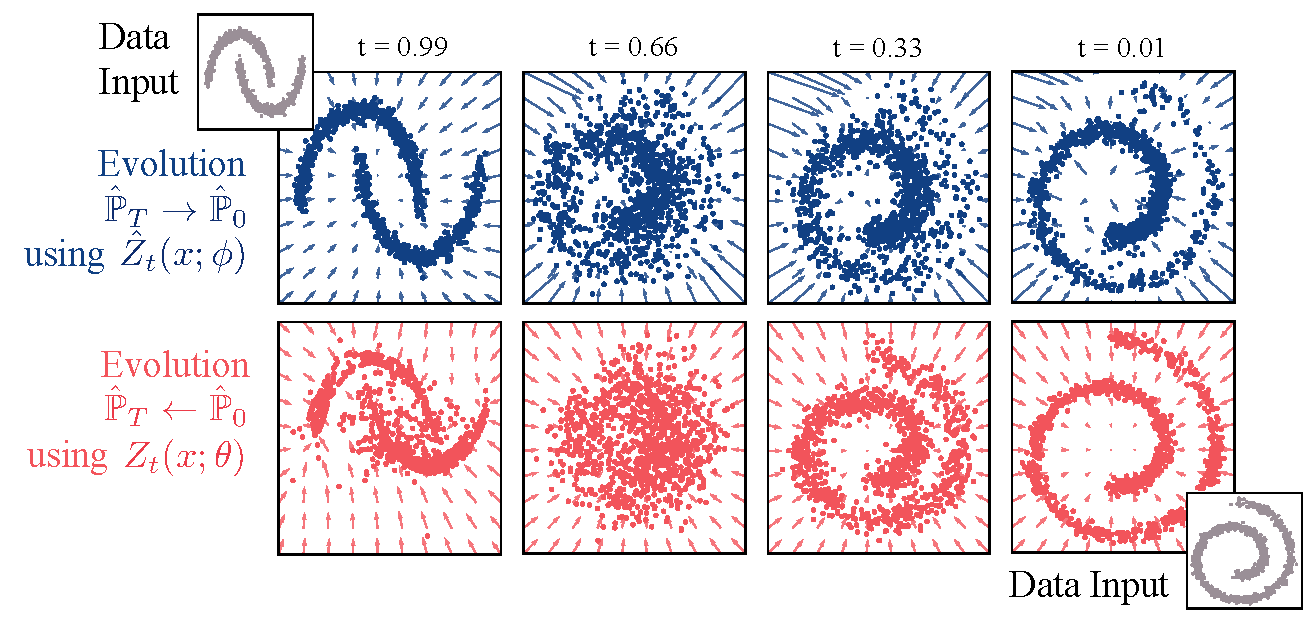
\includegraphics[width=\linewidth]{figures/fig_pred_gsbve_toy_spiral_moon.pdf}
         \caption{Illustration of the time-dependent drifts learned by \textsc{GSBflow} with VE SDE for two toy marginal distributions. \emph{Top.} Evolution of $\distend$ (moons) $\rightarrow \distinit$ (spiral) via backward policy {\color{blue} $\SBb$}. \emph{Bottom.} Evolution of $\distinit$ (spiral) $\rightarrow \distend$ (moons) via forward policy {\color{pink} $\SBf$}.}
        \label{fig:res_synthetic}
\end{figure}

\begin{table}[t]
    \caption{Evaluation of predictive performance w.r.t. the entropy-regularized Wasserstein distance $W_\varepsilon$ \citep{cuturi2013sinkhorn} of \textsc{GSBflow} and baselines on generating different single-cell datasets (using 3 runs).}
    \label{tab:exp_wasserstein_cells}
    \centering
\adjustbox{max width=.99\linewidth}{%
    \begin{tabular}{lcc}
    \toprule
         \textbf{Method} & \multicolumn{2}{c}{\textbf{Tasks}} \\
         & \multicolumn{2}{c}{\makecell{Wasserstein Loss $W_\varepsilon \downarrow$}} \\
         \cmidrule{2-3}
         & \makecell{\citet{moon2019visualizing}} & \makecell{\citet{schiebinger2019optimal}}  \\
    \midrule
      \citet{song2020score} \\
        \tabindent VESDE & $20.83 \pm 0.18$ & $40.81 \pm 0.42$ \\
        \tabindent sub-VPSDE & $\mathbf{19.96 \pm 0.58}$ & $48.15 \pm 3.38$ \\
      \textsc{GSBflow} (\emph{ours}) \\
         \tabindent VESDE & $25.18 \pm 0.10 $ & $\mathbf{27.85 \pm 0.68}$ \\
    \bottomrule
    \end{tabular}
}
\end{table}


The purpose of our experiments is to demonstrate that, by leveraging moment information, \textsc{GSBflow} is significantly more stable compared to other \acrshort{SB}-based objectives, especially when moving beyond the \emph{generative} setting where $\distend$ is a simple Gaussian. Indeed, while performing competitively in the {generative} setting ($\Ncal_0 \rightarrow \distend$), our method \textit{outperforms} when modeling the evolution of two complex distributions ($\distinit \rightarrow \distend$), the most general and ambitious setting to estimate a bridge. This is demonstrated on synthetic data as well as a task from molecular biology concerned with modeling the dynamics of cellular systems, i.e., single-cell genomics \citep{macosko2015highly, frangieh2021multimodal, kulkarni2019beyond}.

\subsubsection{Synthetic Dynamics}

\label{sec:synthetic}
Before conducting the single-cell genomics experiments, we first test \textsc{GSBflow} on a synthetic setting. 
Our first task involves recovering the stochastic evolution of two-dimensional synthetic data containing two interleaving half circles ($\distend$) into a spiral ($\distinit$). 
\cref{fig:res_synthetic} shows the trajectories learned by \textsc{GSBflow} based on the \acrshort{VESDE} (see \cref{tab:examples} and \cref{app:vesde}). 


While it is sufficient to parameterize only a single policy ({\color{blue} $\SBb$}) in generative modeling, the task of learning to evolve $\distinit$ into $\distend$ requires one to recover \emph{both} vector fields {\color{blue} $\SBb$} and {\color{pink} $\SBf$}.
As demonstrated in \cref{fig:res_synthetic}, \textsc{GSBflow} is able to successfully learn both policies {\color{pink} $\SBf$} and {\color{blue} $\SBb$} and reliably recovers the corresponding targets of the forward and backward evolution. While initializing the reference process through the closed-form SB between the Gaussian approximations of both synthetic datasets provides good results, the power of \textsc{GSBflow} becomes evident in more complex applications which we tackle next.


\begin{figure*}
     \centering
         \centering
         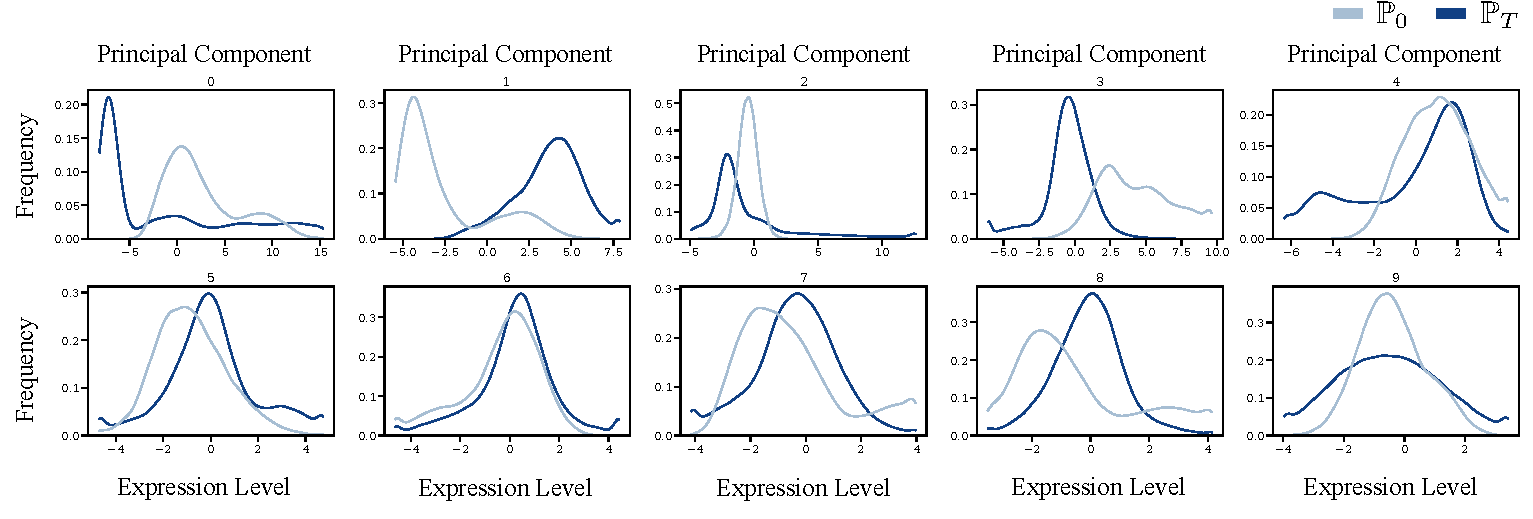
\includegraphics[width=\textwidth]{figures/fig_marginals_schiebinger_pcs_cropped.pdf}
         \caption{The expression levels of the first 10 principal components from the dataset by \citet{schiebinger2019optimal}.}
\label{fig:gaussianMain}
\end{figure*}

\subsubsection{Single-Cell Dynamics}

\looseness -1 Modern single-cell profiling technologies are able to provide rich feature representations (e.g., gene expression) of \textit{individual} cells at any development state. A crucial issue that arises with such profiling methods is their destructive nature: Measuring a cell requires destroying it and thus a cell cannot be measured twice. As a result, independent samples are collected at each snapshot, with no access to ground-truth single-cell trajectories throughout time, resulting in challenging, \emph{unaligned}, datasets.
Recovering cellular dynamics from such unaligned snapshots, i.e., $\distinit$ to $\distend$, has, however, extremely important scientific and biomedical relevance \citep{kulkarni2019beyond}. For example, it determines our understanding on how and why tumor cells evade cancer therapies \citep{frangieh2021multimodal} or unveils mechanisms of cell differentiation and development \citep{schiebinger2019optimal}. Following related work, in particular previous methods based on optimal transport \citep{schiebinger2019optimal, bunne2021learning, bunne2022supervised, tong2020trajectorynet}, the task is thus to learn the stochastic process that described the evolution of single cells from $\distinit$ to $\distend$.

\paragraph{Experimental Setup}

\paragraph{Single-cell genomics via \acrshortpl{SB}}
Let us consider the evolution of a gene, for which we can collect the empirical distributions $\distinit,\distend$ of its expression levels at the times $t=0,1$ \citep{schiebinger2019optimal,moon2019visualizing}. Our goal is to two-fold: 
\begin{enumerate}[itemsep=.0cm,topsep=0cm]
\item To solve the \textbf{generative modeling} problem, i.e., to generate $\distinit$ or $\distend$ from a standard Gaussian noise, and
\item to \textbf{evolve} $\Pinit\to\Pend$ or $\Pend\to\Pinit$, i.e., to recover a stochastic process $\Pmargin$ satisfying $\Pinit = \distinit, \Pend = \distend$.
\end{enumerate}


Although there are numerous algorithms for generative modeling, to our knowledge, the only framework that can simultaneously solve both tasks is the \acrshort{SB}-based scheme recently proposed in \citep{chen2021likelihood}. In order to apply this framework, one has to choose a prior process $\refsde$, which is taken by the authors to be the high-performing \acrshort{VESDE} and sub-\acrshort{VPSDE}. These \acrshort{SB}-based methods, as well as several standard generative modeling algorithms \citep{ho2020denoising, sohl2015deep, song2020score, huang2021variational, song2019generative, song2020score} for the first task, constitute strong baselines for our experiments.

\paragraph{Our choice of $\refsde$; the \textsc{GSBflow}}


Instead of directly diving into the numerical solution of \acrshortpl{SB} as in \citet{chen2021likelihood}, we first empirically verify that the distributions $\distinit,\distend$ in single-cell genomics are typically close to \emph{non-standard} Gaussian distributions: See \cref{fig:gaussianMain} for the canonical dataset \citep{schiebinger2019optimal} and \cref{fig:gaussian} in \cref{app:empirical} for the same phenomenon on another standard benchmark \citep{moon2019visualizing}. 

Since the solutions of \acrshortpl{SB} are Lipschitz in terms of $\distinit,\distend$ \citep{carlier2022lipschitz}, a reasonable approximation to the original \acrshort{SB} objective is to replace $\distinit,\distend$ by Gaussians with matching moments. This results in a \acrshort{GSB} problem which can be solved in closed form by our \cref{thm:GaussianSB}. Intuitively, if we denote an existing prior process by $\refsde$ and the solution of its corresponding \acrshort{GSB} by $\Xsol$, then $\Xsol$ presents a more appealing prior process than $\refsde$ since it carries the moment information of $\distinit$ and $\distend$, whereas $\refsde$ is completely data-oblivious.


Motivated by these observations, we propose a simple modification of the framework in \citet{chen2021likelihood}: Replace the prior process $\refsde$ by its \acrshort{GSB} approximation and keep everything else the same. The resulting scheme, which we term the \textsc{GSBflow}, learns a pair of forward {\color{pink} $\SBf$} and backward parametrized drifts {\color{blue} $\SBb$} that progressively transport samples from $\distinit \rightarrow \distend$ and $\distend \rightarrow \distinit$, respectively. The full algorithm is presented in \cref{sec:methods} for completeness.


\paragraph{Results}
\label{sec:cell}


\begin{figure*}
     \centering
     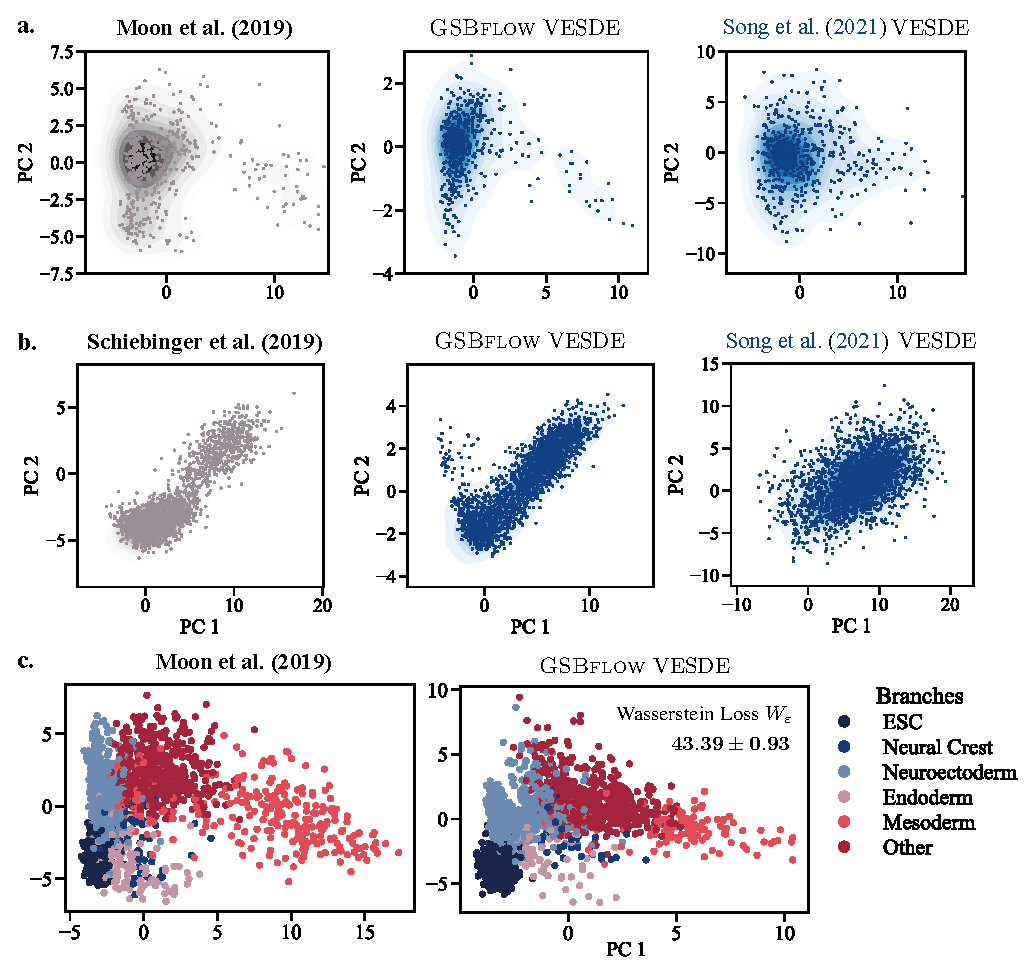
\includegraphics[width=\textwidth]{figures/fig_all_predictions.pdf}
    \caption{\textbf{a.}-\textbf{b.} Visual evaluation of the ability of our method to model the \textbf{generation} of data from \textbf{a.} \citet{moon2019visualizing} and \textbf{b.} \citet{schiebinger2019optimal}. Density plots are visualized in 2D PCA space and show generated data points using either \textsc{GSBflow} (our method) or the procedure in~\citet{song2020score}. \textbf{c.} Evaluation of \textsc{GSBflow}'s ability to model the entire \textbf{evolution} of a developmental process of \citet{moon2019visualizing}, visualized by the data and \textsc{GSBflow} predictions colored by the lineage branch class.}
    \label{fig:all_results}
\end{figure*}

\looseness -1 We investigate the ability of \textsc{GSBflow} to generate cell populations $\distend$ from noise $\Ncal_0$ ($\Ncal_0 \rightarrow \distend$, Fig.~\ref{fig:all_results}a, b) on the the canonical datasets \citep{moon2019visualizing, schiebinger2019optimal}; as well as to predict the dynamics of single-cell genomics ($\distinit \rightarrow \distend$, Fig.~\ref{fig:all_results}c) \citep{moon2019visualizing}, i.e., the inference of cell populations $\distend$ resulting from the developmental process of an initial cell population $\distinit$, with the goal of learning individual dynamics, identify ancestor and descendant cells. Details on datasets and experimental design can be found in \crefrange{app:datasets}{app:experiments}. % In addition, in order to test our hypothesis that the moment information carried by \textsc{GSBflow} leads to a better overall performance, we scale the datasets \citep{moon2019visualizing, schiebinger2019optimal} by 20 and repeat each training procedure.
% We consider the development of human \acrshortpl{ESC} grown as embryoid bodies into diverse cell lineages monitored by single-cell RNA sequencing methods \citep{moon2019visualizing} as well as reprogramming \acrshortpl{MEF} into \acrshortpl{iPSC} \citep{schiebinger2019optimal}.
The evaluation is conducted on the first 20 or 30 components of the PCA space of the >~1500 highly differentiable genes (see \crefrange{fig:moon_expl_variance}{fig:schiebinger_expl_variance}).

\looseness -1 We evaluate the quality of the generated cellular states through the entropy-regularized Wasserstein distance $W_\varepsilon$
% (\texttt{OTT}\footnote{\url{https://github.com/ott-jax/ott}})
(see \cref{tab:exp_wasserstein_cells}) and by visualizing the first two principal components (PC), see \cref{fig:all_results}a,~b.
\textsc{GSBflow} performs competitively on reconstructing embryoid body differentiation landscapes \citep{moon2019visualizing}, and outperforms score-based generative models baselines on the iPSC reprogramming task \citep{schiebinger2019optimal} as quantified by $W_\varepsilon$ between data and predictions.
Further, we analyze \textsc{GSBflow}'s ability to predict the temporal evolution of embryoid body differentiation \citep{moon2019visualizing}, where cells measured at day 1 to 3 serve as samples of $\distinit$, while $\distend$ is constructed from samples between day 12 to 27. As no ground truth trajectories are available in the data, we compare the predicted evolution to the data and compare how well the heterogeneity of lineage (\cref{fig:all_results}c, upper panel) or sublineage branches (\cref{fig:res_evo_subbranches}a) is captured.
\cref{fig:all_results}c (lower panel) and \cref{fig:res_evo_subbranches}b thereby closely resemble the data (see $W_\varepsilon$ in \cref{fig:all_results}c) and thus demonstrate \textsc{GSBflow}'s ability to learn cell differentiation into various lineages and to capture biological heterogeneity on a more macroscopic level.


\subsection{Discussion}
\looseness -1 We derive closed-form solutions of \acrshortpl{GSB}, an important class of dynamic \acrshort{OT} problems. Our technique originates from a deep connection between Gaussian \acrshort{OT} and the Bures-Wasserstein geometry, which we generalize to the case of general \acrshort{SB} problems. Numerically, we demonstrate that our new closed forms inspire a simple modification of existing \acrshort{SB}-based numerical schemes, which can however lead to significantly improved performance.

\textbf{Limitation of our framework. }
\looseness -1 In a broader context, we hope our results can serve as the inspiration for more learning algorithms, much like how existing closed-form solutions of Gaussian \acrshort{OT} problems have contributed to the machine learning community. We thus acknowledge a severe limitation of our closed-form solutions: These formulas require matrix inversions, which might face scalability issues for high-dimensional data. In addition, existing matrix inversion algorithms are typically extremely sensitive to the condition number, and thus our formulas are not as useful for ill-conditioned data. Lifting these constraints to facilitate further applications, such as to image datasets, is an important future work.

